\section{Abstract smooth surfaces}

\subsection{Charts and atlases}
Recall that if $\Sigma$ is a topological surface, any point lies in an open neighbourhood homeomorphic to a disc.

\begin{definition}[Chart]
	A pair $(U, \varphi)$, where $U$ is an open set in $\Sigma$ and $\varphi \colon U \to V$ is a homeomorphism to an open set $V \subseteq \mathbb R^2$, is called a \vocab{chart} for $\Sigma$.
	If $p \in U$, we might say that $(U, \varphi)$ is a chart for $\Sigma$ \textit{at $p$}.
\end{definition}

\begin{definition}[Local parameterisation]
	The inverse $\sigma = \varphi^{-1} \colon V \to U$ is known as a \vocab{local parametrisation} for the surface.
\end{definition} 

\begin{definition}[Atlas]
	A collection of charts $\{ (U_i, \phi_i)_{i \in I}\}$ whose domains cover $\Sigma$ ($\cup_{i \in I} U_i = \Sigma$) is known as an \vocab{atlas} for $\Sigma$.
\end{definition} 

\begin{example}
	If $Z \subseteq \mathbb R^2$ is closed, $\mathbb R^2 \setminus Z$ is a topological surface with an atlas containing one chart, $(\mathbb R^2 \setminus Z, \phi = \id)$.
\end{example}

\begin{example}
	For $S^2$, there is an atlas with two charts, which are the two stereographic projections from the poles.
	% We could consider alternative charts, for instance the projection to the $yz$ plane, but this would be insufficient for describing the poles.
\end{example} 

\begin{definition}[Transition Map]
	Let $(U_i, \varphi_i)$ be charts containing the point $p \in \Sigma$, for $i = 1, 2$.
	Then the map
	\begin{align*}
		\varphi_2 \circ \eval{\varphi_1^{-1}}_{\varphi_1(U_1 \cap U_2)} : \varphi_1(U_1 \cap U_2) \to \varphi_2(U_1 \cap U_2)
	\end{align*}
	converts between the corresponding charts, and is called a \vocab{transition map} between charts.
	This is a homeomorphism of open sets in $\mathbb R^2$.
\end{definition}

\begin{figure}[h] 
    \centering 
    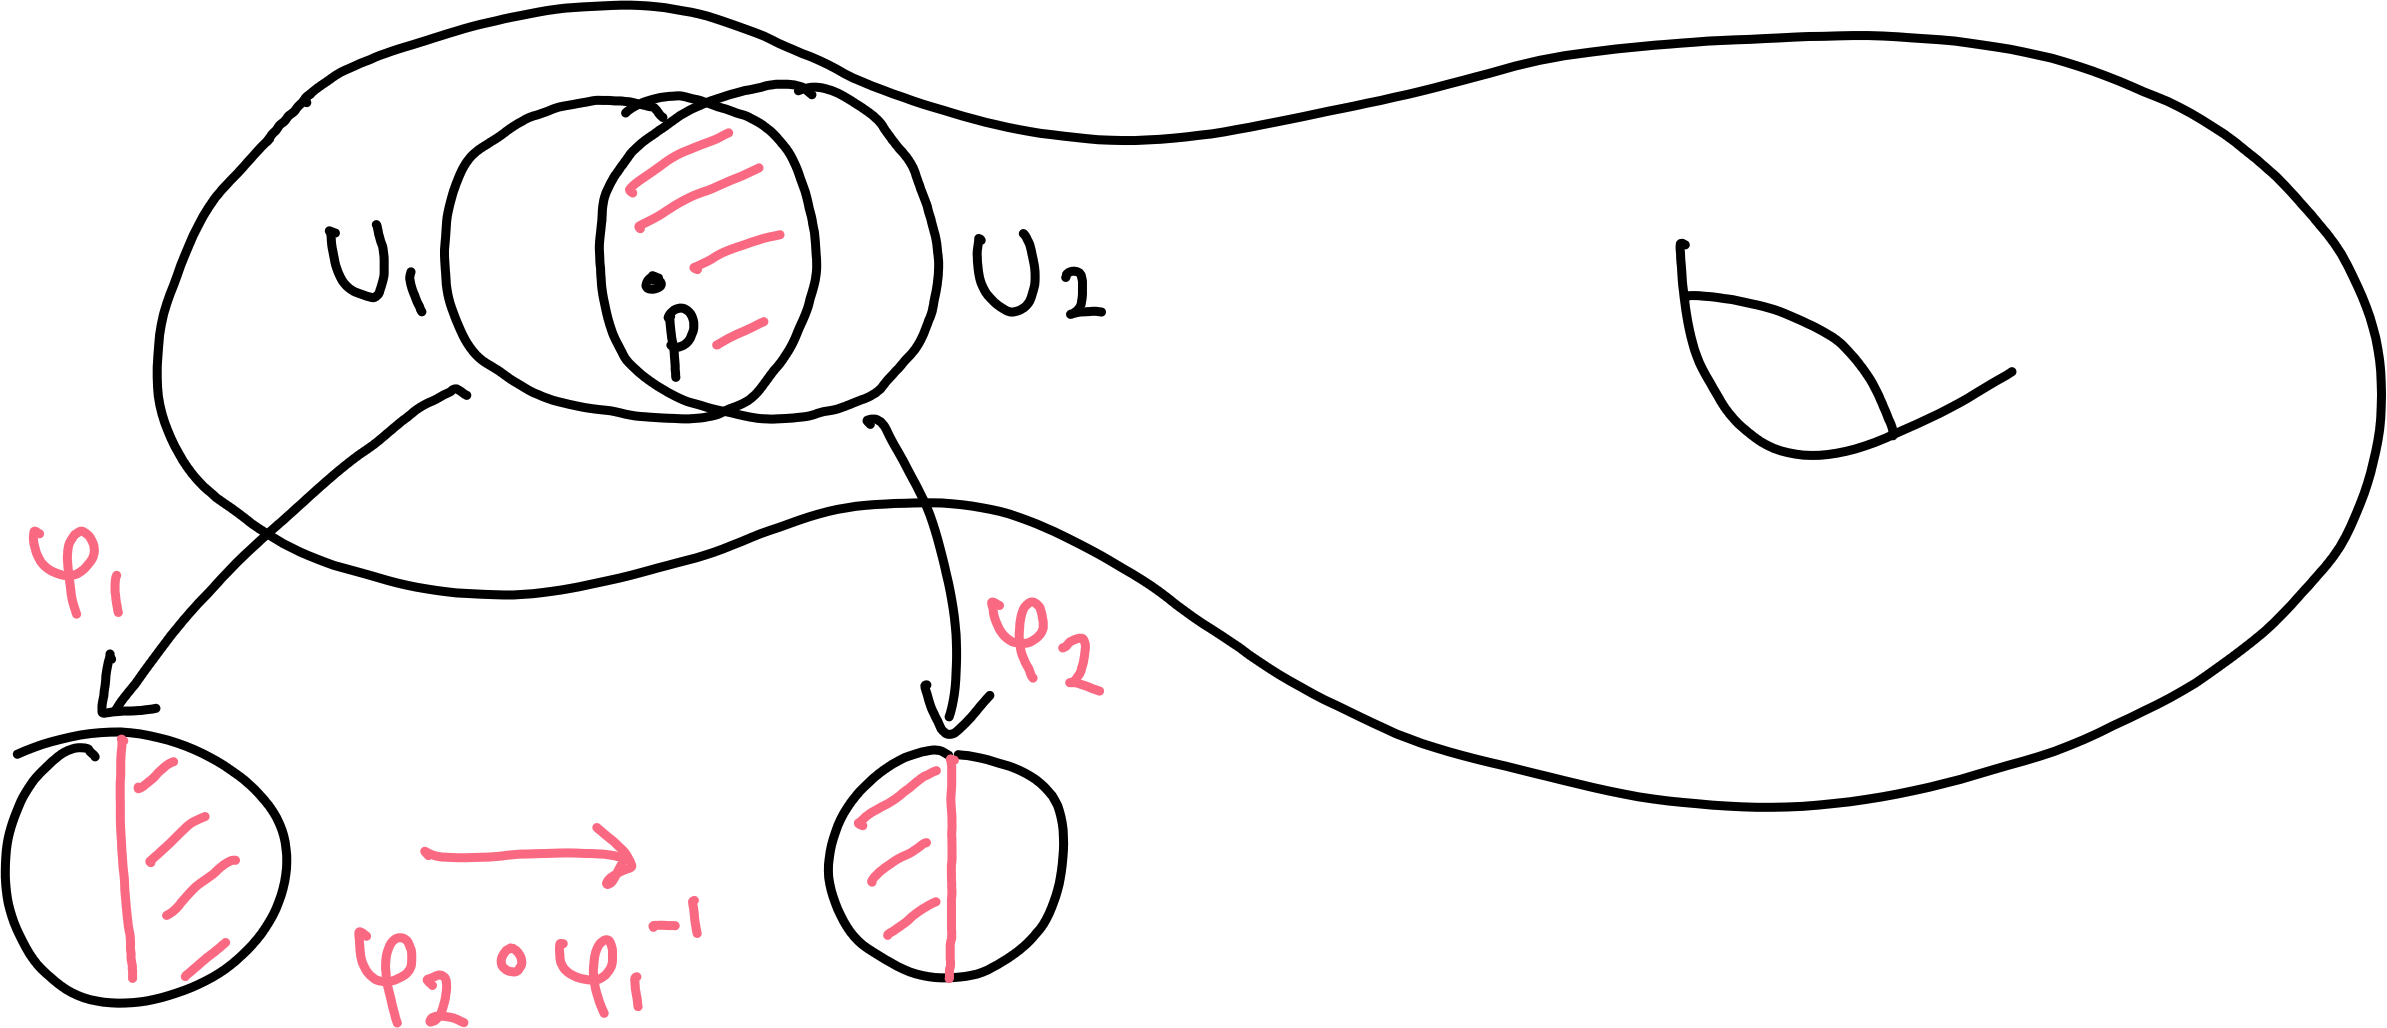
\includegraphics[height=5cm]{02-transition} 
\end{figure}

Recall from Analysis and Topology that if $V \subseteq \mathbb R^n$ and $V' \subseteq \mathbb R^m$ are open, then a continuous map $f \colon V \to V'$ is called \textit{smooth} if it is infinitely differentiable.
Equivalently, it is smooth if continuous partial derivatives of all orders in all variables exist at all points.

\begin{definition}[Diffeomorphism]
	A homeomorphism $f : V \to V'$ is called a \vocab{diffeomorphism} if it is smooth and it has a smooth inverse.
\end{definition} 

\begin{definition}[Abstract Smooth Surface]
	An \vocab{abstract smooth surface} $\Sigma$ is a topological space with an atlas of charts $\{(U_i, \varphi_i)_{i \in I}\}$ s.t. all transition maps are diffeomorphisms.
\end{definition}

\begin{remark}
	We could not simply consider a smoothness condition for $\Sigma$ itself without appealing to atlases, since $\Sigma$ is an arbitrary topological space and could have almost any topology.
\end{remark}

\begin{example}
	The atlas of two charts with stereographic projections gives $S^2$ the structure of an abstract smooth surface.
\end{example}

\begin{example}
	For the torus $T^2 = \faktor{\mathbb R^2}{\mathbb Z^2}$, recall that we obtained charts from (the inverses of) the projection restricted to small discs in $\mathbb{R}^2$.

	The transition maps for this atlas are all translations\footnote{If small discs intersect in $\faktor{\mathbb R^2}{\mathbb Z^2}$ then they have points which are integer translations?} of $\mathbb R^2$.
	Hence $T^2$ inherits the structure of an abstract smooth surface.
	Explicitly, let us define $e \colon \mathbb R^2 \to T^2$ by $(t,s) \mapsto \qty(e^{2\pi i t}, e^{2 \pi i s})$, then consider the atlas
	\begin{align*}
		\qty{(e\qty(D_\varepsilon(x,y)), e^{-1} \text{ on this image})}
	\end{align*}
	for $\varepsilon < \frac{1}{3}$.
	These are charts on $T^2$, and the transition maps are (restricted to appropriate domains) translations in $\mathbb R^2$.
	Hence $T^2$, via this atlas, has the structure of an abstract smooth surface.
\end{example}

\begin{remark}
	The definition of a topological surface is a notion of structure.
	One can observe a topological space and determine whether it is a topological surface.
	Conversely, to be an abstract smooth surface is to have a specific set of data; that is, we must provide charts for the surface in order to see that it is indeed an abstract smooth surface.
\end{remark}

\begin{definition}[Smooth Function]
	Let $\Sigma$ be an abstract smooth surface, and $f \colon \Sigma \to \mathbb R^n$ be a continuous map.
	We say that $f$ is \vocab{smooth} at $p \in \Sigma$ if, for all charts $(U, \varphi)$ of $p$\footnote{$p \in U$} belonging to the smooth atlas for $\Sigma$, the map
	\begin{align*}
		f \circ \varphi^{-1} \colon \underbracket{\varphi(U)}_{\subset \mathbb{R}^2} \to \mathbb R^n
	\end{align*}
	is smooth at $\varphi(p) \in \mathbb R^2$.
\end{definition}

\begin{figure}[h] 
    \centering 
    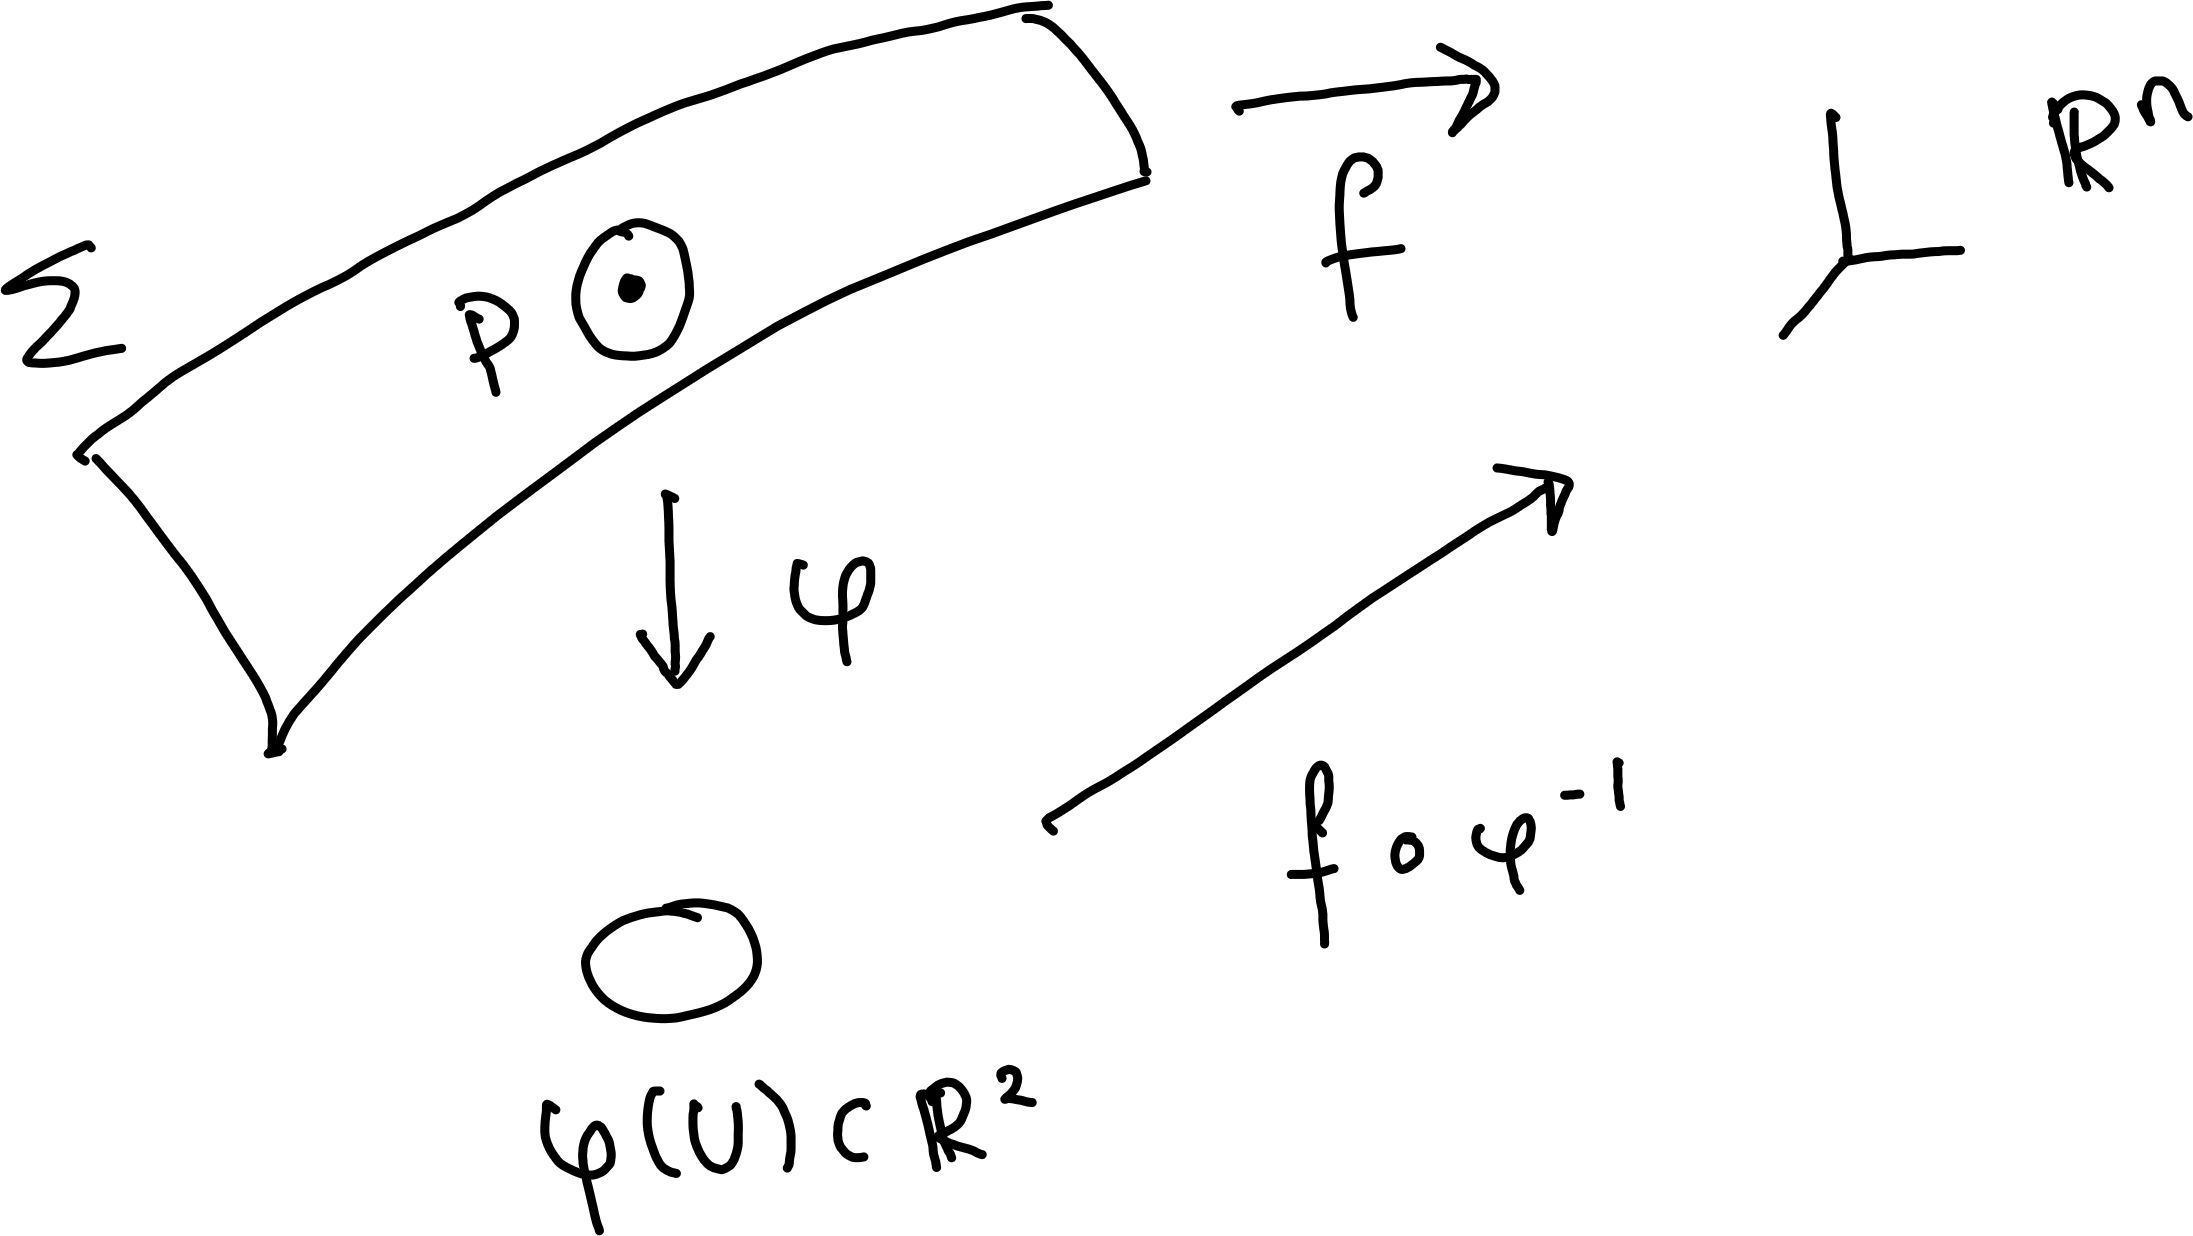
\includegraphics[height=5cm]{02-smoothfunction} 
\end{figure}

\begin{remark}
	Note that the choice of chart and atlas was arbitrary, but smoothness of $f$ at $p$ is independent of the choice of chart, since the transition maps between two such charts are diffeomorphisms.
	\begin{align*}
		f \circ \phi_1\inv &= f \circ \phi_2\inv \circ (\phi_2 \circ \phi_1\inv)
	\end{align*} 
	$(\phi_2 \circ \phi_1\inv)$ is a transition map and so is a diffeomorphism. So by chain rule follows!
\end{remark}

\begin{definition}[Smooth Function between Surfaces]
	Let $\Sigma_1, \Sigma_2$ be abstract smooth surfaces. \\
	Then a map $f \colon \Sigma_1 \to \Sigma_2$ is \vocab{smooth} if it is `smooth in the local charts'.
	Given a chart $(U, \varphi)$ at $p$ and a chart $(U', \psi)$ at $f(p)$, with $f(U) \subset U'$, the map $\psi \circ f \circ \varphi^{-1}$ is smooth at $\varphi(p)$.
\end{definition}

\begin{figure}[h] 
    \centering 
    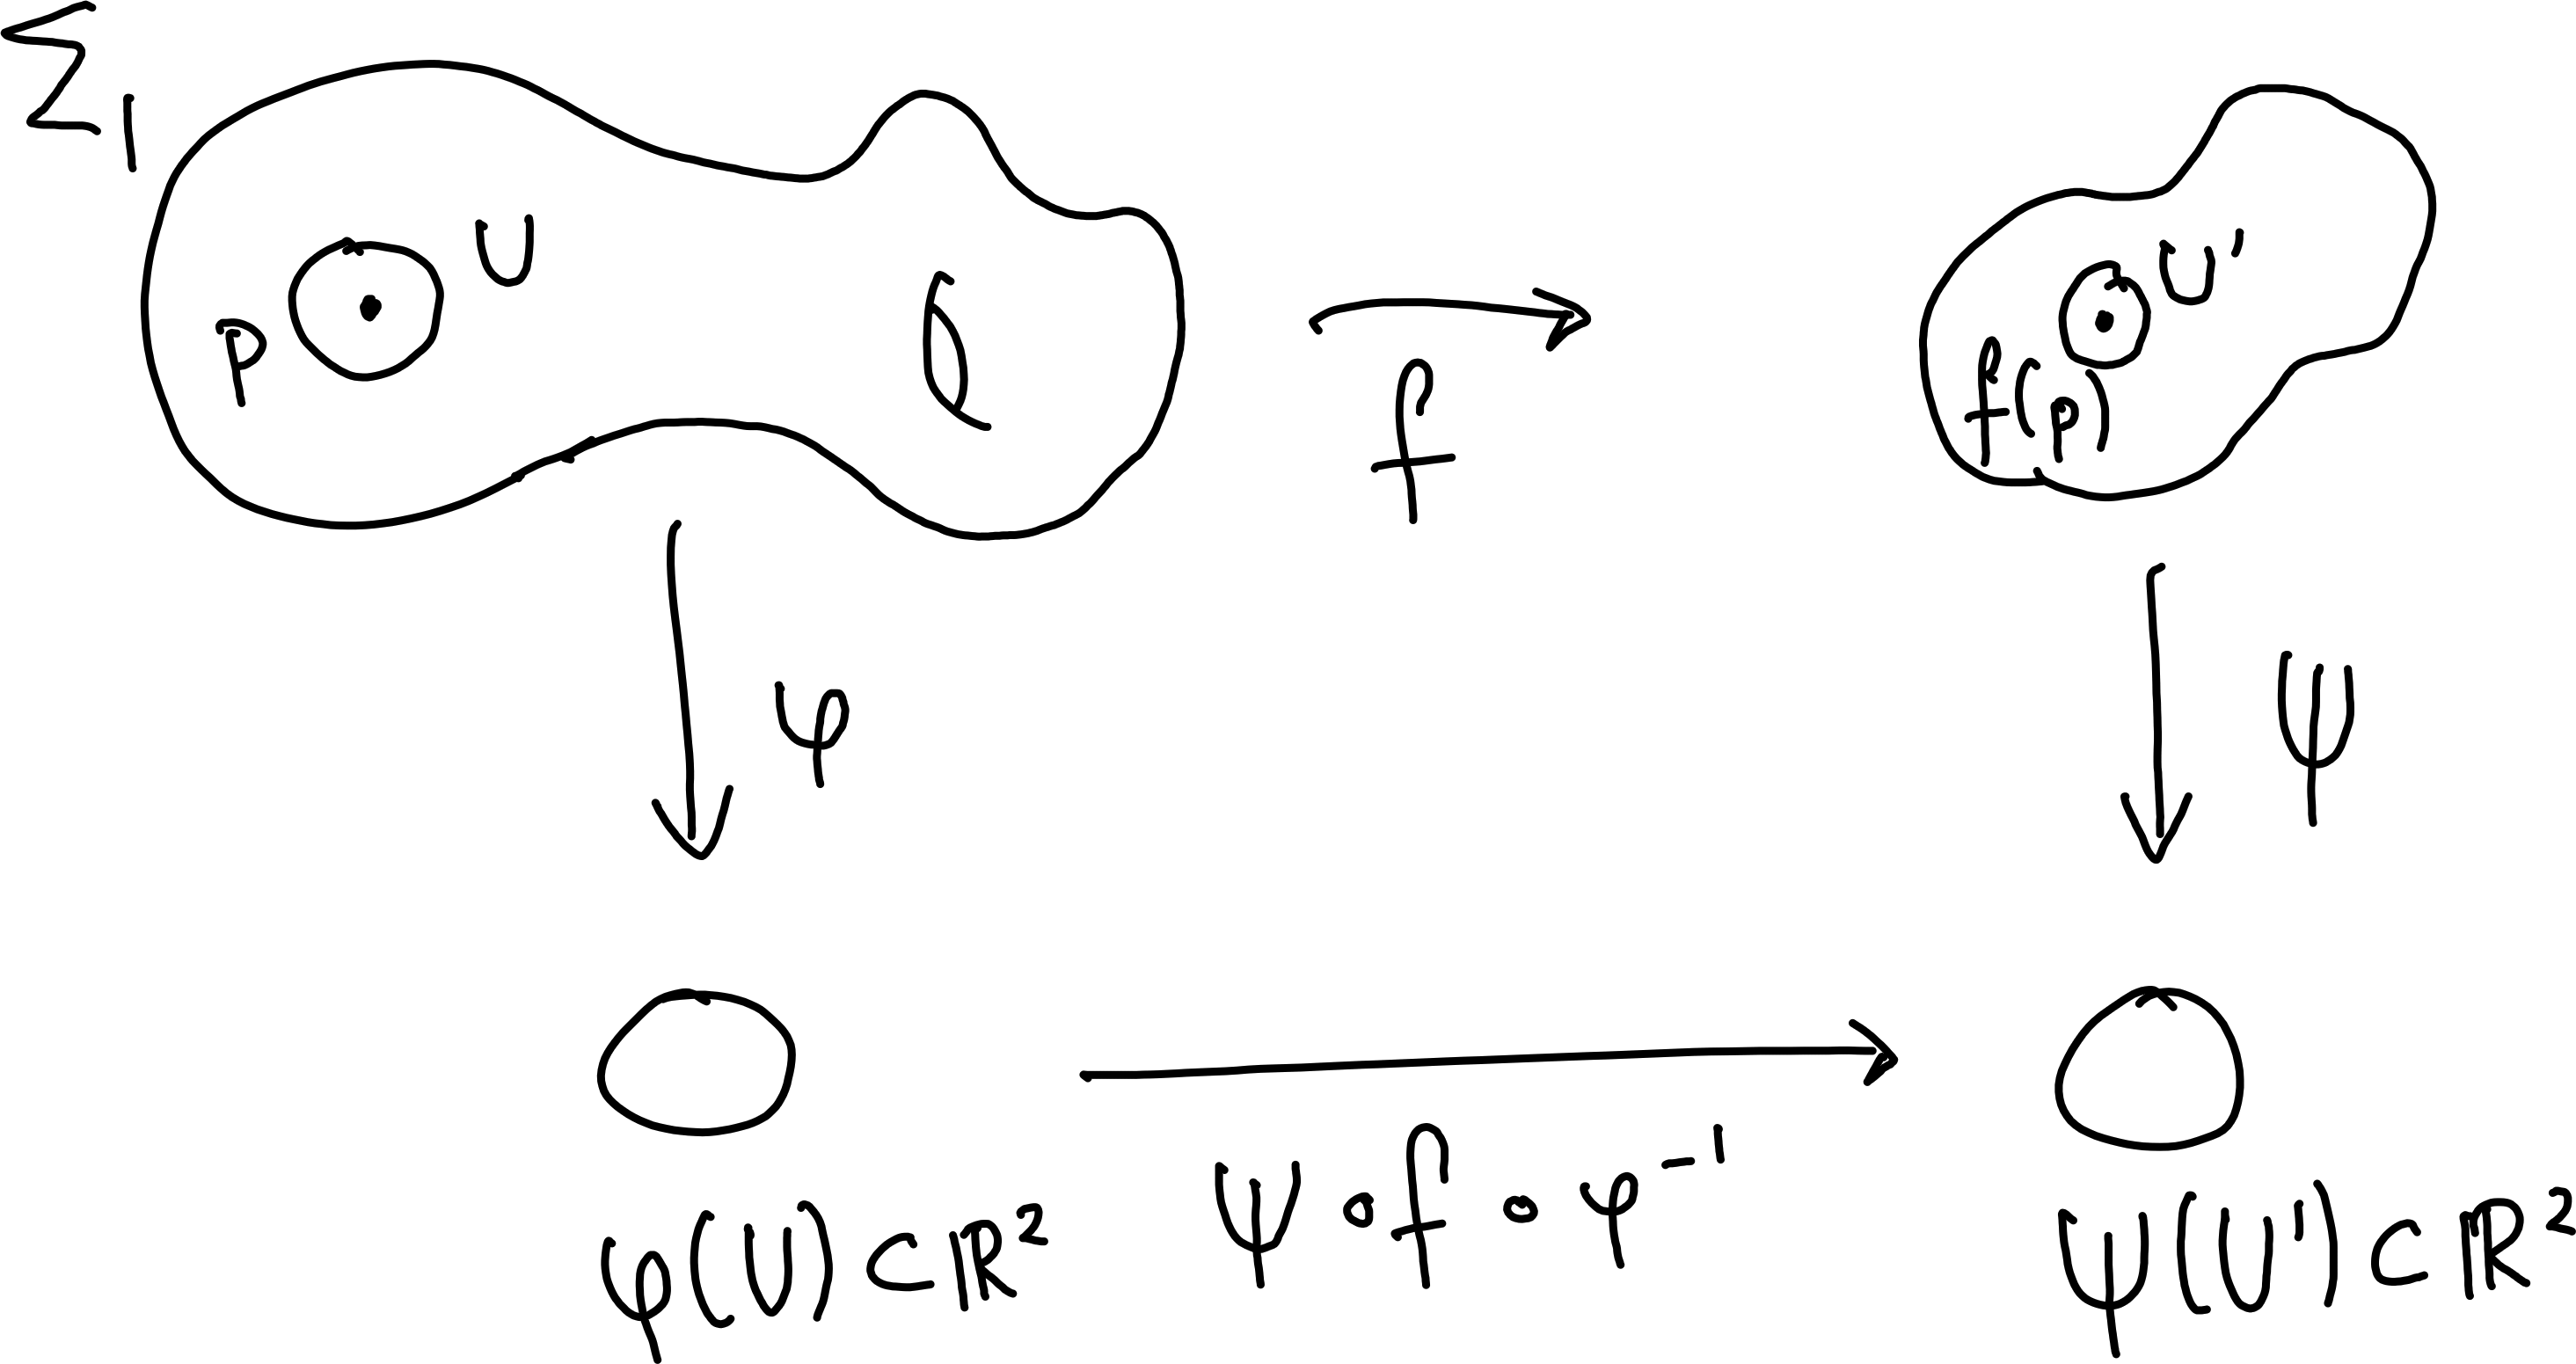
\includegraphics[height=5cm]{02-smoothfunctionbetweensurfaces} 
\end{figure}

\begin{remark}
	Smoothness of $f$ at $p$ does not depend on the choice of chart, provided that the charts all belong to the same atlas.
\end{remark} 

\begin{definition}[Diffeomorphic Surfaces]
	Two surfaces $\Sigma_1, \Sigma_2$ are \vocab{diffeomorphic} if $\exists \; f \colon \Sigma_1 \to \Sigma_2$ which is smooth and has smooth inverse.
\end{definition}

\begin{remark}
	Often, we convert from a given smooth atlas for an abstract smooth surface $\Sigma$ to the \textit{maximal compatible} smooth atlas.
	That is, we consider the atlas with the maximal possible set of charts, all of which have transition maps that are diffeomorphisms.
	This can be accomplished formally by use of Zorn's lemma.
\end{remark}
